\section{Identification and Removal of Runtime Inefficiencies}
\label{removal}

The identification and removal of inefficiencies follows the same iterative approach presented in section \ref{identification}.

\subsection{First Iteration}

Without the sensibility provided by the tests in section \ref{identification}, a scientist would incur in the pitfall of using all available cores (and even all hardware threads) on the system hoping that it would provide the best performance. While it may be true for the non-pointer implementation, it would inefficiently use the system computational resources, and using the single device highly efficient pointer implementation would provide a even greater waste.

Since the pointer implementation is the most efficient but only when using a single device, using multiple processes may provide better efficiency. As it was not possible to refactor LipMiniAnalysis to change the event information from a global to a private state, an MPI implementation was discarded due to the communication overhead necessary in each event processing.

A characteristic of particle reconstructions at CERN is that the processing is made by executing the application on a vast set of 1GB input files. The system resources can be efficiently used if it is performed a careful balancing of the input files across a set of application processes, producing the same goal of an MPI implementation but with no need for communicating between processes. A dispatcher was devised, which takes a set of input files and creates a given amount of \tth processes. It is then responsible for dispatching the files to the different processes in a queue-like approach, and monitors their execution. A set of 20 input files was considered for testing purposes, with different configurations of processes and threads per process.

\begin{figure}[!htp]
	\begin{center}
		\raisebox{-0.5\height}{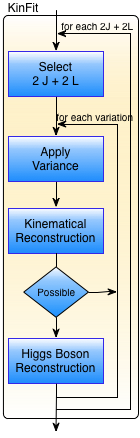
\includegraphics[scale=0.7]{images/sequential_kinfit.png}}
		\raisebox{-0.5\height}{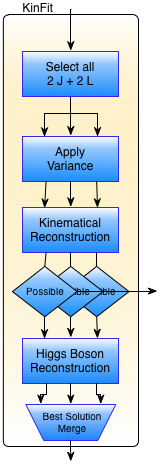
\includegraphics[scale=0.7]{images/parallel_kinfit.png}}
		\caption{Schematic representation of the \ttDilepKinFit sequential (left) and parallel (right) workflows.}
		\label{fig:Sched}
	\end{center}
\end{figure}

Figure \ref{fig:Sched} presents the speedups using 2, 4, 5, 8, and 10 processes for different thread configurations to fill one or both CPU devices.

\begin{itemize}
	\item At runtime
	\begin{itemize}
		\item Thread affinity experiments vs standard OpenMP affinity (force bad affinity examples that may occur to compare the performance?)
		\item Using all available cores is not always profitable
		\item Many processes/threads combinations, also testing thread affinity
	\end{itemize}
\end{itemize}
